\num{5} Leia o texto.

\begin{quote}
\textbf{Vacinação infantil sofre queda brusca no Brasil}

A baixa cobertura vacinal no país deixa a população infantil exposta a
doenças que antes não eram mais uma preocupação, como o sarampo, que foi
erradicado no país em 2016 e em 2018 voltou para a lista de doenças no
Brasil. Além do sarampo, outras doenças que correm o risco de voltar a
acometer as crianças são a poliomielite, meningite, rubéola e a
difteria.

{[}...{]}

Maria Luiza La Porta e Everton Lima. IFF/Fiocruz -- Instituto Fernandes
Figueira/Fundação Osvaldo Cruz. Vacinação infantil sofre queda brusca no
Brasil. \fonte{Disponível em:
\textit{https://portal.fiocruz.br/noticia/vacinacao-infantil-sofre-queda-brusca-no-brasil}.
Acesso em: 21 abr. 2023.}
\end{quote}

O texto revela que

\begin{escolha}
\item não há vacinas para diversas doenças nos postos de saúde do Brasil.

\item todas as crianças brasileiras estão protegidas contra várias doenças.

\item diminuiu o número de crianças vacinadas em todo o território nacional.

\item a poliomielite e outras doenças estão completamente afastadas do país.
\end{escolha}


\num{6} Leia o texto com atenção.

\begin{quote}
\textbf{De mãos dadas com os povos originários}

{[}...{]}

Desde 1500, a população indígena não cresce. Pelo contrário, ela só
diminui. Será que os povos indígenas foram reduzindo como mágica? Não
mesmo. {[}...{]} os motivos são muitos. Mas o pior deles talvez seja o
apagamento de sua história. Faz ideia do que seja isso?

O apagamento histórico dos indígenas começa quando são tratados como
selvagens; quando não se compreende a cultura, a crença, as tradições,
os costumes e lhes chamam de atrasados ou inferiores; ou quando invadem
suas terras e se pratica todo tipo de violência contra homens, mulheres
e crianças.

{[}...{]}

Bianca Encarnação e Cathia Abreu (Instituto Ciência Hoje) e Marcos
Rodrigues Barreto (Fundação Municipal de Educação de Niterói). CHC --
Ciência Hoje das Crianças. De mãos dadas com os povos originários.
\fonte{Disponível em:
\textit{https://chc.org.br/artigo/de-maos-dadas-com-os-povos-originarios/}
. Acesso em: 21 abr. 2023.}
\end{quote}

De acordo com o texto,

\begin{escolha}
\item a população indígena é cada vez maior porque compreendemos sua cultura.

\item a redução dos povos indígenas acontece pela magia que eles dominam.

\item um dos motivos da diminuição de indígenas é o apagamento de sua história.

\item o crescimento da população indígena está ligado a suas crenças e tradições.
\end{escolha}


\num{7} Preste atenção no diálogo a seguir.

\begin{quote}
Olívia: Oi! Tudo bem? Não posso ir a sua casa na quinta. Vou dar plantão
no hospital. Desculpe!

Sara: Ah, que pena! Mas tudo bem. Bom trabalho.

Olívia: Obrigada. Posso passar aí no sábado? A gente papeia e pede uma
pizza.

Sara: Claro. Até sábado. Beijos.

Olívia: Beijos.

\fonte{Texto escrito para este material.}
\end{quote}

Qual informação não está explícita nesse texto, mas é possível de ser
deduzida?

\begin{escolha}
\item Olívia é médica-chefe do hospital em que vai dar plantão.

\item O diálogo entre as amigas aconteceu em uma terça-feira.

\item Sara não trabalha e, por isso, poderia se encontrar na quinta.

\item Olívia e Sara tinham combinado de se encontrar na sexta.
\end{escolha}


\num{8} Leia o texto.

\begin{quote}
\textbf{Chuvas torrenciais serão cada vez mais frequentes, dizem
meteorologistas}

As chuvas torrenciais que provocaram a morte de mais de 50 pessoas no
litoral norte de São Paulo devem ser cada vez mais frequentes no Brasil
e no mundo graças ao aquecimento global, afirmam meteorologistas
consultados {[}...{]}.

{[}...{]} A quantidade de chuva foi considerada um novo recorde no
Brasil, superando a tragédia em Petrópolis {[}em 2022{]}.

{[}...{]}

Wanderley Preite Sobrinho. Chuvas torrenciais serão cada vez mais
frequentes, dizem meteorologistas. UOL Notícias. \fonte{Disponível em:
\textit{https://noticias.uol.com.br/cotidiano/ultimas-noticias/2023/02/25/eventos-extremos-aquecimento-global-chuvas-litoral-norte-de-sao-paulo.htm}.
Acesso em: 21 abr. 2023.}
\end{quote}

Mesmo que não se conheçam todas as palavras, o que se entende do texto?

\begin{escolha}
\item As chuvas em Petrópolis foram mais fortes que as que caíram em São Paulo.

\item As chuvas no litoral de São Paulo foram as mais fortes já registradas no Brasil.

\item Chuvas como as de Petrópolis foram causadas pelo derretimento das geleiras.

\item Chuvas como as do litoral de São Paulo cairão uma vez por ano no Brasil.
\end{escolha}



\num{9} Leia as frases a seguir e identifique aquela que apresenta palavra
com sufixo que indica diminutivo e palavra com prefixo que indica
anterioridade.

\begin{escolha}
\item O passarinho que nasceu anteontem já está tentando voar.

\item A escola vai completar a montagem do parquinho à tarde.

\item É uma tristeza ver o desmatamento de florestas nativas.

\item O chuvisco que caiu hoje cedo ajudou a limpar o ar.
\end{escolha}


\num{10} Analise a imagem e identifique a que gênero ela se relaciona.

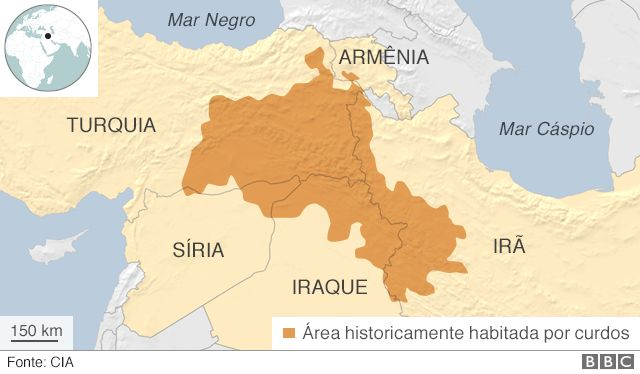
\includegraphics[width=1.84348in,height=1.84348in]{media/image1.jpeg}


O texto dramático requer encenação, pode provocar diversas reações como
riso, choro, surpresa, raiva e medo e tem características próprias,
diferentes de outros gêneros textuais, como

\begin{escolha}
\item ser dividido em atos e cenas, geralmente em ordem cronológica.

\item precisar de pelo menos dois atores ou atrizes para ser encenado.

\item não necessitar descrever o contexto em que a situação vai acontecer.

\item necessitar de narrador para conduzir o enredo e apresentar os personagens.
\end{escolha}



\num{11} Leia o texto atentamente.

\begin{quote}
Em uma noite muito, mas muito fria, um morador de rua que não tinha para
onde ir, vestindo apenas uma camiseta de mangas curtas e calça comprida
já remendada, implorava por agasalho a todos que passavam pelo local.

\fonte{Texto escrito para este material.}
\end{quote}

A maneira de falar do morador de rua, expressa no verbo de enunciação,
permite compreender que ele:

\begin{escolha}
\item desejava ardentemente um agasalho.

\item precisava demasiadamente de um agasalho.

\item queria insistentemente um agasalho.

\item exigia incansavelmente um agalho.
\end{escolha}



\num{12} No discurso direto, o sinal de pontuação a ser utilizado no início
de uma frase para indicar que um personagem vai falar

\begin{escolha}
\item são os parênteses.

\item são os dois-pontos.

\item é o ponto de interrogação.

\item é o travessão.
\end{escolha}


\num{13} Observe atentamente a peça publicitária que fez parte de campanha do
Governo do Distrito Federal contra a dengue.

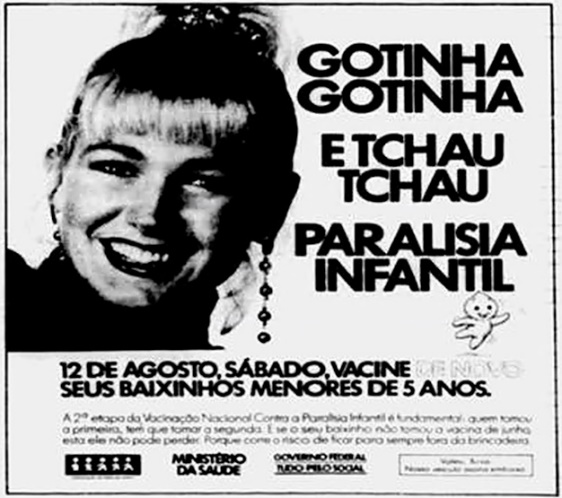
\includegraphics[width=2.34792in,height=3.28681in]{media/image2.jpeg}

%\textit{https://www.comunicacao.df.gov.br/campanha-de-combate-a-dengue/}

O jogo de palavras utilizado no pôster para chamar a atenção do público
(adultos, adolescentes e crianças) foi:

\begin{escolha}
\item Guerra contra a dengue. Juntos, somos mais fortes.

\item Família nota 10 não hospeda o mosquito \emph{Aedes aegypti}.

\item Evite água parada. Proteja sua família.

\item Feche bem o saco de lixo e deixe-o fora do alcance de animais.
\end{escolha}


\num{14} Leia o texto.

\begin{verse}
A jovem pianista é uma flor\\
Que despertou o meu amor.\\
Com as crianças é bondosa.\\
Com os idosos, atenciosa.\\
Tem sempre muita alegria\\
Que a todos contagia.\\
\fonte{Texto escrito para este material.}
\end{verse}

O sentido figurado, muitas vezes utilizado em poemas para criar imagens
que ajudem o leitor a compreender a ideia que se pretende transmitir,
pode ser reconhecido no seguinte verso:

\begin{escolha}
\item Com os idosos, atenciosa.

\item Que a todos contagia.

\item A jovem pianista é uma flor

\item Despertou o meu amor.
\end{escolha}



\num{15} Leia o texto.

Uma turma combinou de almoçar às 12 horas para despedir-se do amigo que
ia estudar na Europa. Rodolfo, um dos convidados, chegou às 14 e foi
recebido com a seguinte frase: ``Oi, Rodolfo! Chegou cedo para o jantar.
Vai almoçar? Tomar alguma coisa?''.

Texto escrito para este material.

O uso do advérbio ``cedo'' cria uma

\begin{escolha}
\item ironia.

\item incoerência.

\item ambiguidade.

\item incompreensão.
\end{escolha}



\section{SIMULADO 2}\label{simulado-2}

\num{5} Leia as frases observando a colocação dos adjetivos.

1) Eis o meu velho cachorro.

2) Eis o meu cachorro velho.

3) Este é um grande homem.

4) Este é um homem grande.

Os sentidos dos adjetivos em cada frase são, respectivamente,

\begin{escolha}
\item companheiro antigo --- idoso --- notável --- alto

\item brincalhão --- companheiro antigo --- rico --- alto

\item inteligente --- companheiro antigo --- alto --- respeitável

\item companheiro antigo --- inteligente --- notável --- rico
\end{escolha}



\num{6} A língua sofre constantes, porém não repentinas, mutações. Essas
variações linguísticas têm diversas causas e ocorrem em todos os
lugares, não apenas no Brasil. Leia os exemplos a seguir.

1) Vossa mercê --- vosmecê --- você;

2) Boticário --- farmacêutico;

3) Ela é uma gata --- ela é muito bonita.

As variações linguísticas apresentadas referem-se a:

\begin{escolha}
\item diferenças de acordo com a região.

\item mudanças com o passar do tempo.

\item vocabulário de grupos sociais distintos.

\item estilo conforme a situação --- formal/informal.
\end{escolha}



\num{7} Leia o poema.

Sissi sai, sibila, silva

Sissi sai, essência sente

Sissi sai, senso, centelha

Sissi sai, Sissi a serpente.

Texto escrito para este material.

Qual é a principal marca do poema apresentado?

\begin{escolha}
\item Harmonia por meio de rimas intercaladas.

\item Imagem poética por meio de metáfora.

\item Efeito sonoro por meio de aliteração.

\item Força pela repetição do fonema S.
\end{escolha}


\num{8} Leio o texto.

\textbf{Clima já mudou, e adaptação é urgente, afirmam especialistas}

{[}...{]}

Nos últimos anos, recorrentes alertas dos pesquisadores do Painel
Intergovernamental de Mudanças Climáticas (IPCC) da Organização das
Nações Unidas (ONU) indicaram que a influência humana levou o planeta à
trajetória de aquecimento mais rápida em 2 mil anos e já produziu uma
temperatura média que supera o período pré-industrial em mais de 1 grau
Celsius (°C).

{[}...{]}

O secretário executivo do Observatório do Clima, Marcio Astrini,
ressalta que houve uma sucessão de eventos extremos nos últimos anos,
incluindo temporais no Recife, na Bahia e no norte de Minas Gerais.
Segundo Astrini, a comprovação de que um evento específico está
relacionado às mudanças climáticas é uma conclusão que nem sempre fica
clara, mas o acúmulo de eventos como esses já é considerado consequência
das alterações no clima por especialistas.

{[}...{]}

Vinícius Lisboa. Agência Brasil -- Rio de Janeiro. Clima já mudou, e
adaptação é urgente, dizem especialistas.
\textit{https://agenciabrasil.ebc.com.br/geral/noticia/2023-02/clima-ja-mudou-e-adaptacao-e-urgente-afirmam-especialistas}.Acesso
em 21 abr. 2023.

O texto chama a atenção para o fato de que

\begin{escolha}
\item as mudanças climáticas são consequência direta da ação do ser humano e de que deve haver ações contra isso.

\item os temporais e outros eventos extremos deixarão de ocorrer espontaneamente.

\item a geografia de alguns estados brasileiros é responsável pela ocorrência de temporais.

\item a possibilidade de eventos climáticos serem naturais é real, desconectados da interferência humana.
\end{escolha}


\num{9} Leia o texto.

Manual para montagem de brinquedos, receita de bolo, bula de remédio:
são gêneros textuais do tipo injuntivo, que fazem parte do dia a dia de
praticamente toda a população.

Que característica pode marcar textos desse tipo?

\begin{escolha}
\item Uso do imperativo.

\item Presença de narrador.

\item Utilização de adjetivos.

\item Exposição de fatos.
\end{escolha}


\num{10} Leia o texto.

\textbf{O leão}

Na imensa planície africana, existia um leão com dentes enormes e
afiados. Chamava-se Praxedes. Era só o Praxedes abrir sua boca, balançar
a densa juba e fazer explodir seu urro, ouvido a 50 quilômetros de
distância, para que toda a floresta tremesse de medo. Os macacos
trepavam até os galhos mais altos, as hienas paravam de sorrir e corriam
mais do que os veados, os outros leões abaixavam a cabeça e enfiavam o
rabo entre as pernas.

Com o Praxedes era na base: obediência ou morte!

--- Sim, Dom Praxedes.

--- Tá certo! É o senhor quem manda.

--- Se Dom Praxedes não quer, eu não faço.

{[}...{]}

Tarcísio Lage. O leão Praxedes. \fonte{Disponível em:
\textit{http://www.dominiopublico.gov.br/download/texto/ea000464.pdf}.
Acesso em: 22 abr. 2023.

Os principais elementos do texto narrativo como o que você acabou de ler
são:

\begin{escolha}
\item verbos sempre no presente, discursos direto e indireto, adjetivos, fatos e opiniões.

\item verbos em qualquer tempo, discurso direto, presença de narrador, locuções adverbiais.

\item verbos no futuro, ausência de diálogos, histórias sempre fictícias, discurso indireto.

\item verbos normalmente no passado, personagens, espaço definido, narrador, ação.
\end{escolha}


\num{11} Preste atenção nas frases a seguir.

1) Meu irmãozinho nasceu!

2) Tem uma aranha enorme na cozinha!

3) Que dia lindo!

4) Não acredito que você teve a coragem de fazer isso comigo!

As frases têm em comum o ponto de exclamação, mas cada uma revela uma
sensação, que, na ordem, são

\begin{escolha}
\item tristeza, desprezo, alegria e medo.

\item admiração, indignação, susto e alívio

\item alegria, susto, admiração e indignação.

\item Medo, tristeza, alívio e raiva.
\end{escolha}


\num{12} Observe o anúncio.

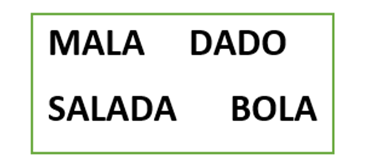
\includegraphics[width=5.90556in,height=2.72153in]{media/image3.png}

https://www.gov.br/saude/pt-br/assuntos/noticias/2023/fevereiro/ministerio-da-saude-lanca-movimento-nacional-pela-vacinacao

A grande quantidade de cores no anúncio pode estar relacionada ao fato
de que a campanha de vacinação

\begin{escolha}
\item atende a apenas parte do território.

\item objetiva atingir apenas uma parcela da população.

\item pretende ser uma celebração da vida.

\item volta-se somente para o público infantil.
\end{escolha}



\num{13} O sufixo ``-ão'' ligado a substantivos e adjetivos pode ser
empregado para formar novas palavras no grau aumentativo. Pensando
nisso, observe as palavras a seguir.

Cirurgião

Macarrão

Mão

Paizão

Porção

Tubarão

Entre essas palavras, a formada por esse sufixo é

\begin{escolha}
\item ``cirurgião''.

\item ``mão''.

\item ``paizão''.

\item ``tubarão''.
\end{escolha}


\num{14} Leia o texto.

{[}...{]}. E eu estava me lembrando de uma música que Mamãe cantava
quando eu era bem pequenino. Ela ficava no tanque, com um pano amarrado
na cabeça para tapar o sol. Tinha um avental amarrado na barriga e
ficava horas e horas, metendo a mão na água, fazendo sabão virar muita
espuma. Depois torcida a roupa e ia até a corda. Prendia tudo na corda e
suspendia o bambu. Ela fazia igualzinho com todas as roupas. Estava
lavando a roupa da casa do Dr. Faulhaber para ajudar nas despesas da
casa. {[}...{]}

José Mauro de Vasconcelos. Meu pé de laranja lima. Editora
Melhoramentos. Livro digital publicado em 26 de março de 2013.
\fonte{Disponível em:
\textit{https://www.google.com.br/books/edition/O_meu_p\%C3\%A9_de_laranja_lima_Edi\%C3\%A7\%C3\%A3o_hist/8AOIYOdyt1wC?hl=pt-BR\&gbpv=1\&printsec=frontcover}
Acesso em: 21 abr. 2023.

A partir desse fragmento do romance \emph{Meu pé de laranja lima}, é
possível afirmar que

\begin{escolha}
\item Mamãe cantava porque seu sonho era tornar-se cantora.

\item Mamãe lavava as roupas do Dr. Faulhaber rapidamente.

\item Mamãe cantava para encantar quem estivesse por perto.

\item Mamãe lavava roupa para contribuir com o sustento da família.
\end{escolha}


15. Leia o texto.

\textbf{Educação financeira: como e quando começar?}

De acordo com especialista, crianças devem saber a real importância do
dinheiro, desde a primeira vez que lhe é dado algum valor.

O doutor em Finanças, Moisés Silva Martins, ressalta que {[}...{]} ``Se
a criança aprende a não gastar com coisas supérfluas o dinheiro que
recebe dos pais, quando ela trabalhar vai entender e valorizar seu
salário'' {[}...{]}.

Coluna Espaço Infantil. O Imparcial. Educação financeira: como e quando
começar? \fonte{Disponível em:
\textit{https://www.imparcial.com.br/noticias/educacao-financeira-como-e-quando-comecar,28939}.
Acesso em: 23 abr. 2023.

No texto acima, os argumentos do especialista contribuem para que

\begin{escolha}
\item se confie nas informações, já que ele conhece o assunto.

\item os pais pensem em fazer poupança para seus filhos.

\item os pais incentivem as crianças a gastarem o dinheiro que ganham.

\item não se confie nas informações, já que não se sabe se são verdadeiras.
\end{escolha}


\section{SIMULADO 3}\label{simulado-3}

5) Observe o texto não verbal.

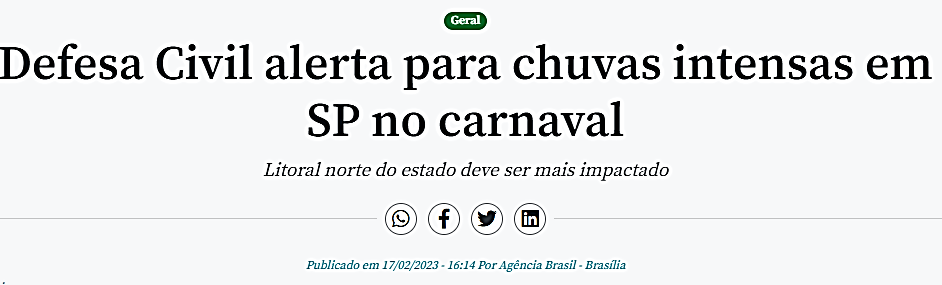
\includegraphics[width=4.21875in,height=4.21875in]{media/image4.png}

\fonte{Disponível em
\textit{https://pixabay.com/pt/illustrations/res\%c3\%adduos-de-pl\%c3\%a1stico-oceano-polui\%c3\%a7\%c3\%a3o-7617451/}.
Acesso em 23 abr. 2023

Mesmo sem contar com palavras, é possível entender que a mensagem
implícita no texto é

\begin{escolha}
\item a beleza dos habitantes do mundo marinho nacional.

\item a proteção que garrafas plásticas proporcionam aos peixes.

\item a poluição de rios e mares com resíduos plásticos.

\item a diversidade da flora e da fauna aquáticas brasileiras.
\end{escolha}



6) Leia o texto.

\textsc{Skate para crianças: montado e novinho}

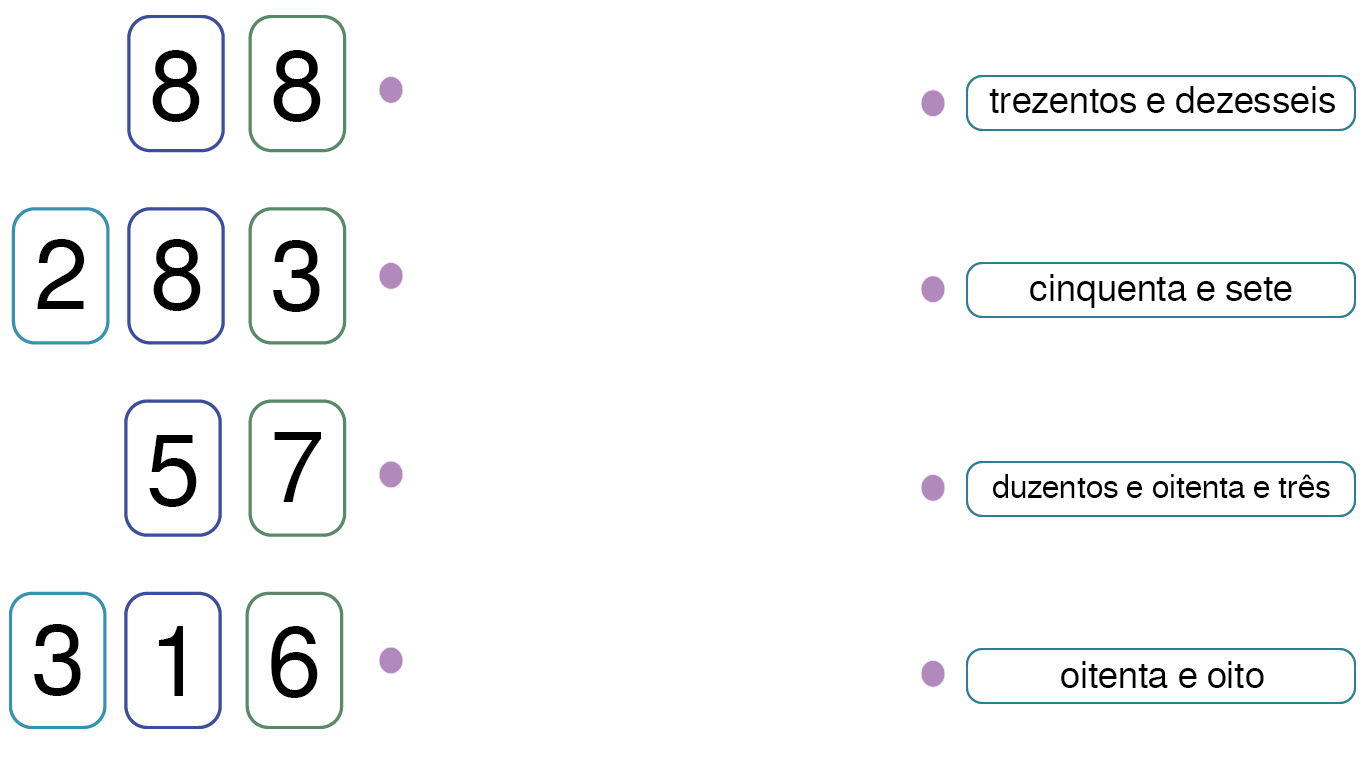
\includegraphics[width=5.25000in,height=3.47639in]{media/image5.png}

\fonte{Disponível em
\textit{https://www.pexels.com/pt-br/foto/fotografia-com-foco-raso-de-skate-marrom-e-azul-1018484/}.
Acesso em 23 abr. 2023.

O skate Irado da marca Radicais é ideal para crianças de 7 a 9 anos.
Rápido e estável em curvas e retas. Produzido com madeira Maple, tem
17,8 cm x 18,1 cm, rodas vermelhas e amortecedores para dar total
segurança aos pequenos. O modelo à venda tem linda decoração exclusiva
na parte de baixo criada pelo artista australiano John Stevaux. Valor
promocional para o mês de dezembro: R\$2.000,00. Pagamento: PIX,
dinheiro ou cartão de débito com 10\% de desconto, além de cartão de
crédito. Enviamos para todo o Brasil.

Contato:
\textit{skatistadahora@manobrasradicais.com.br} / WhatsApp: (22) 99999-0000

(Texto criado pela autora especialmente para este material)

Esse tipo de anúncio aparece em diversos veículos de comunicação; por
isso, recebe o nome de \emph{Anúncio Classificado}. Sua principal função
é vender ou alugar alguma coisa e, para isso, utiliza-se de

\begin{escolha}
\item argumentação histórica.

\item descrição.

\item narração.

\item dissertação.
\end{escolha}


7) Conto ou não conto?

{[}...{]}

A minha língua coçou. Um segredo daqueles não poderia ficar guardado. Na
primeira oportunidade em que eu fiquei sozinha, procurei minha tia, que
estava preparando o almoço.

-- Tia, preciso contar uma coisa pra senhora.

-- Pois conte, que estou ouvindo. Não posso te dar mais atenção, senão o
almoço não sai...

-- É que eu tenho um segredo pra te contar e não sei se devo...

-- O segredo é seu ou dos outros?

-- Dos outros... Quer dizer, da prima!

-- E por que você quer contar os segredos alheios?

-- Bem, eu pensei que a senhora quisesse saber o que aconteceu...

-- Ah, minha filha, deixa eu te fazer apenas uma pergunta: a dona do
segredo te autorizou a contá-lo?

-- Na verdade, não!

-- E por qual motivo você me contaria, então?

-- É que... Bem, o que ela fez não é muito certo...

{[}...{]}

Abel Sidney. Conto ou não conto? \fonte{Disponível em
\textit{http://www.dominiopublico.gov.br/download/texto/ea000337.pdf} .
Acesso em 23 abr. 2023

Nesse texto, em que a história é contada em primeira pessoa, o narrador
é

\begin{escolha}
\item a sobrinha.

\item a tia.

\item a prima.

\item um personagem externo à história.
\end{escolha}


8) Preste atenção ao texto.

Personagens

\emph{Sabrina}: garotinha de 5 anos; cabelos na altura do ombro, loiros
e cacheados; olhos castanhos e atentos; bochechas rosadas de tanto
correr. Está descalça e usa um vestido florido.

\emph{Mamãe}: mulher de 33 anos; loira; olhos azuis; voz calma; trabalha
cuidando da casa, da família e dos animais de estimação. Usa um vestido
simples, na altura dos joelhos, e chinelos. Seus lindos cabelos
cacheados estão presos em um coque.

\emph{Papai}: homem de 31 anos; cabelos castanho claros, lisos e curtos,
arrumados com gel; olhos castanhos; bigode em que fica mexendo quando
está pensando em como resolver alguma coisa. Veste uma calça de moletom,
camiseta e chinelos.

Cena 1:

É um sábado. Mamãe e Papai estão sentados lado a lado no sofá da sala
fazendo planos para o domingo. De repente, Sabrina entra subitamente na
sala, ofegante porque acabara de correr para contar o que tinha
acontecido. Como estava visivelmente feliz, Mamãe e Papai não se
preocuparam e aguardaram, com leve sorriso, que ela se recuperasse para
começar a falar.

-- Mamãe, papai (vai andando até perto do sofá). Vocês não vão acreditar
(abre um imenso sorriso) acabei de ver a fada do dente no quintal.

Papai levanta rapidamente e, dando a mão para a Mamãe se levantar
também, exclama: -- Nossa, que bacana!!! Eu também quero ver. Onde ela
está? (vai caminhando em direção à porta).

(Material criado pela autora exclusivamente para este material)

Os elementos acima são marcas específicas do

\begin{escolha}
\item texto dramático.

\item poema concreto.

\item texto publicitário.

\item conto realista.
\end{escolha}

9) Leia o texto.

\section{Cão é resgatado após passar três dias em poço de 15m de
profundidade em Itapipoca, no
Ceará}\label{cuxe3o-uxe9-resgatado-apuxf3s-passar-truxeas-dias-em-pouxe7o-de-15m-de-profundidade-em-itapipoca-no-cearuxe1}

\subsection{\texorpdfstring{\emph{O caso aconteceu na localidade de
Galego, zona rural do
município.}}{O caso aconteceu na localidade de Galego, zona rural do município.}}\label{o-caso-aconteceu-na-localidade-de-galego-zona-rural-do-municuxedpio.}

Um cão foi resgatado após cair e passar três dias em um poço com cerca
de 15 metros de profundidade em
Itapipoca, na
região norte do Ceará. O resgate foi realizado pelo Corpo de Bombeiros
na zona rural do município.

{[}...{]}

g1 Ceará -- Cão é resgatado após passar três dias em poço de 15m de
profundidade em Itapipoca, no Ceará. \fonte{Disponível em
\textit{https://g1.globo.com/ce/ceara/noticia/2023/04/23/cao-e-resgatado-apos-passar-tres-dias-em-poco-de-15m-de-profundidade-em-itapipoca-no-ceara.ghtml}.
Acesso em 23 abr. 2023.

O gênero textual jornalístico apresentado é

\begin{escolha}
\item uma charge.

\item uma notícia.

\item um artigo de opinião.

\item uma reportagem.
\end{escolha}

10) --- Acabei de fazer a lista do supermercado: maçã, laranja, alface,
tomate, berinjela, aveia, iogurte natural, arroz e café.

--- Nossa! Já? Como você foi rápida!

Nesse pequeno diálogo, vírgula e ponto de exclamação foram utilizados,
respectivamente, para

\begin{escolha}
\item separar termos enumerados; expressar surpresa.

\item separar vocativo; expressar susto.

\item separar sujeito de predicado; expressar indignação.

\item separar conjunções; expressar alegria.
\end{escolha}

11) Observe o diálogo.

--- Humm... estou sentindo um cheirinho de macaxeira. Adoroooo!

--- Que estranho. O cheiro que estou sentindo é de aipim.

--- Uai... Para mim cheiro é de mandioca.

Os três amigos resolveram ir atrás do cheiro e, quando descobriram que
era a mesma coisa, caíram na gargalhada.

que esse tubérculo é conhecido por diferentes nomes em diferentes
estados e regiões do Brasil.

A variedade linguística identificada no diálogo é do tipo

\begin{escolha}
\item histórica.

\item geográfica.

\item social.

\item situacional.
\end{escolha}

12) Leia o texto.

Ninguém sabia onde estava Marcos. Procura daqui, procura dali... e
acabaram por achá-lo à beira do lago que atravessa a cidade. Os amigos,
que já andavam preocupados, ficaram tranquilos quando o avistaram.
Porém, quando se aproximaram, perceberam que ele chorava copiosamente
--- e um deles perguntou:

--- Marcos, o que houve?

Com muito esforço, ele conteve as lágrimas e contou o que aconteceu:

--- A Bambina, minha cachorrinha, sempre vai me encontrar na saída da
escola... e hoje não foi. Chamei, mas infelizmente ela não apareceu.
Estranhei, mas comecei a fazer o caminho de volta pra casa. Já andei
atrás dela no bairro todo. Ninguém viu a Bambina. Ela é minha
com-pa-nhei-ra --- disse o rapaz, com a voz entrecortada porque
recomeçou a chorar.

(Material elaborado pela autora para utilização neste material)

Marcos não estava apenas triste, mas desesperado, com o sumiço da
Bambina. Isso pode ser percebido pela utilização do advérbio

\begin{escolha}
\item preocupados.

\item sempre.

\item copiosamente.

\item infelizmente.
\end{escolha}
13) Leia o texto.

A quermesse estava ótima. Muita música, quadrilha, barracas de
brincadeiras, bebidas, comidinhas bem gostosas, e doces, principalmente
os caseiros --- de abóbora, de coco e de leite ---, divinos.

A intenção do autor ao colocar travessões no meio da frase foi

\begin{escolha}
\item cortar a sentença, que estava muito longa.

\item dar destaque aos diversos doces caseiros.

\item separar os diversos doces dos salgados.

\item mostrar que, na quermesse, havia doces caseiros.
\end{escolha}
14) Observe o anúncio.

\fonte{Disponível em
\textit{https://www.navegantes.sc.gov.br/noticia/17090/campanha-dezembro-verde-alerta-sobre-abandono-de-animais}.
Acesso em 23 abr. 2023

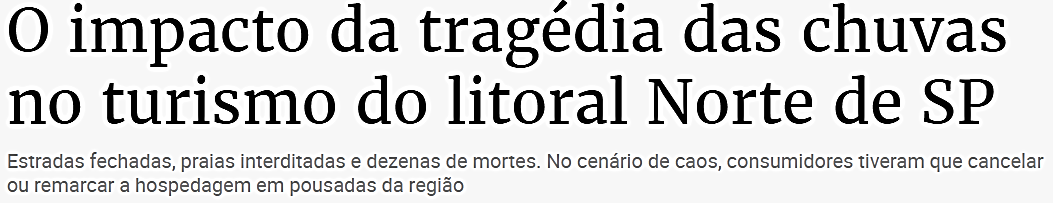
\includegraphics[width=4.50972in,height=4.50972in]{media/image6.png}

O principal elemento persuasivo do anúncio é

\begin{escolha}
\item a frase ``Diga não ao abandono de animais''.

\item o apoio da Prefeitura de Navegantes à campanha.

\item a frase ``Ele faz parte das suas escolhas''.

\item a foto do cãozinho abandonado na estrada.
\end{escolha}


15) Leia o texto.

Sou meio arredondada e pequena. Por dentro sou amarelinha bem clarinha e
por fora posso ser verde, amarela ou vermelhinha. Algumas vezes sou doce
e outras, azedinha. Não sou muito dura, mas também não sou molinha.
Posso virar suco, geleia, bolo e tortinha. Sou muito apreciada no Brasil
e em praticamente todo o mundo.

A esta altura você já sabe que o texto fala de maçã, e descobriu isso
pela presença de adjetivos, sem os quais seria impossível descrever a
fruta. Um desses adjetivos é

\begin{escolha}
\item dentro.

\item azedinha.

\item praticamente.

\item posso.
\end{escolha}

\section{SIMULADO 4}\label{simulado-4}

5. Leia o texto.

Joana era nutricionista de uma empresa, mas perdeu o emprego durante a
pandemia e já estava há mais de dois anos sem trabalhar. Fazia um
servicinho aqui, outro ali, para conseguir levar algum dinheiro para
casa e ajudar nas despesas.

Como ela sempre foi boa funcionária, um dia, ela recebeu o telefonema de
um antigo chefe perguntando se ela teria interesse em atuar como
nutricionista de uma escola. Ela aceitou a oferta e agarrou a
oportunidade com unhas e dentes, objetivando guardar dinheiro e
contribuir com a família para comprar uma casa.

Texto escrito para este material.

A expressão ``agarrar com unhas e dentes'' significa

\begin{escolha}
\item esforçar-se ao máximo para não perder o novo emprego.

\item descansar para recomeçar a procura mais tarde.

\item partir para a briga para conseguir o que se deseja.

\item seguir em frente, apesar dos momentos difíceis.
\end{escolha}

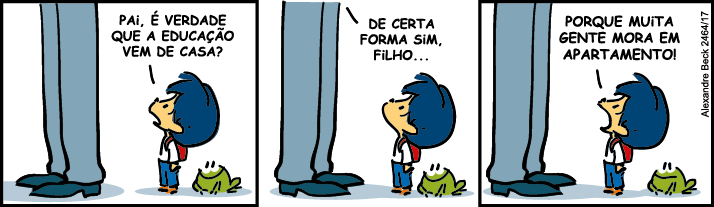
\includegraphics[width=2.43333in,height=3.24514in]{media/image7.png}6.
Analise cuidadosamente o infográfico a seguir.

\textit{https://www.gov.br/pt-br/noticias/transito-e-transportes/2021/04/programa-ja-instalou-mais-de-13-2-mil-pontos-de-internet-no-pais}

Esse texto foi elaborado pelo Ministério das Comunicações utilizando
vários elementos com a intenção de transmitir a ideia central com
clareza: onde estão os pontos instalados do programa Wi-Fi Brasil. Por
meio desse material, entendemos que o estado e o local mais beneficiados
foram

\begin{escolha}
\item o Maranhão e as unidades de saúde.

\item o Ceará e os telecentros.

\item a Bahia e as escolas.

\item o Amazonas e as comunidades indígenas.
\end{escolha}

7. Leia o texto.

\textbf{``Lá vem história'': por que é saudável ler para crianças?}

\emph{Além de ser um exercício que desperta o encantamento, estudos
apontam que ler em voz alta para crianças é fundamental para o
desenvolvimento da linguagem}

{[}...{]}

O artigo ``Aprender a partir da leitura em voz alta dos adultos'',
publicado pelas pesquisadoras Ana Teberosky e Angelica Sepúlveda, da
Universidade de Barcelona, na Espanha, confirma a riqueza de
aprendizados gerados a partir da leitura de histórias {[}...{]}.

{[}...{]}

As autoras defendem que essa escuta leva {[}à{]} construção de um
vocabulário mais rico e ao desenvolvimento de uma linguagem mais
complexa e elaborada pelos pequenos.

Lunetas. ``Lá vem história'': por que é saudável ler para crianças?
\fonte{Disponível em: \textit{https://lunetas.com.br/ler-para-criancas/} . Acesso
em: 24 abr. 2023.

O artigo publicado pelas pesquisadoras da Universidade de Barcelona

\begin{escolha}
\item combate a ideia de que é bom ler em voz alta para crianças.

\item nega que as crianças desenvolvam uma linguagem mais complexa.

\item deixa dúvidas se faz bem ler em voz alta para crianças.

\item reforça a importância de ler em voz alta para crianças.
\end{escolha}


\num{8} Observe os dois textos reproduzidos a seguir.

\textbf{Recomece}

{[}...{]}

Quando tudo for escuro

e nada iluminar,

quando tudo for incerto

e você só duvidar...

É hora do recomeço.

Recomece a ACREDITAR.

{[}...{]}

Bráulio Bessa. Recomece. \fonte{Disponível em
\textit{https://www.brauliobessa.com/post/recomece}. Acesso em 24 abr. 2023

\textbf{O guardador de rebanhos}

Eu nunca guardei rebanhos,

Mas é como se os guardasse.

Minha alma é como um pastor,

Conhece o vento e o sol

E anda pela mão das Estações

A seguir e a olhar.

Toda a paz da Natureza sem gente

Vem sentar-se a meu lado.

Mas eu fico triste como um pôr de sol

Para a nossa imaginação,

Quando esfria no fundo da planície

E se sente a noite entrada

Como uma borboleta pela janela.

{[}...{]}

Alberto Caeiro (heterônimo de Fernando Pessoa). O guardador de rebanhos.
\fonte{Disponível em:
\textit{http://www.dominiopublico.gov.br/download/texto/pe000001.pdf}.
Acesso em: 25 abr. 2023.

Os dois textos são trechos de poemas, respectivamente, com 6 e 13
versos. Outra diferença é que o

\begin{escolha}
\item primeiro tem rimas e o segundo não.

\item primeiro tem estrofe e o segundo não.

\item segundo tem rimas e o primeiro não.

\item segundo tem estrofe e o primeiro não.
\end{escolha}


\num{9} Leia o parágrafo.

Os microplásticos podem ter diferentes origens. Uma delas é a degradação
de plásticos maiores que, com o tempo, fragmentam-se em pedaços cada vez
menores por conta da ação de raios ultravioleta, ondas e o atrito com
areias e pedras.

Julia di Spagna. Guia do Estudante. Microplásticos: entenda os impactos
no meio ambiente e na saúde humana. \fonte{Disponível em:
\textit{https://guiadoestudante.abril.com.br/atualidades/o-que-sao-microplasticos-e-o-impacto-no-meio-ambiente-e-na-saude-humana/}.
Acesso em: 25 abr. 2023.

Uma palavra do texto formada por um prefixo que indica diminutivo é

\begin{escolha}
\item ``ultravioleta''.

\item ``degradação''.

\item ``microplásticos''.

\item ``maiores''.
\end{escolha}


\num{10} Leia o texto.

25/04/2023

Hoje assisti a um filme muito legal que se passava na Grécia, um país
muito, mas muito antigo mesmo, que fica na Europa. Lá tem praias lindas,
muito azuis, e diversos museus --- eu adoro museus! E tem
construções muito antigas... pena que algumas delas estão meio
destruídas.

O filme mostra que os gregos são muito alegres, estão sempre cantando e
dançando. E têm um costume diferente: em festas de casamentos, eles
jogam pratos no chão para quebrá-los... dizem que é para dar sorte aos
noivos.

E as comidas também parecem muito gostosas, como o mussaká, que é tipo
uma lasanha de berinjela.

Ah, e como a Grécia é formada por várias ilhas, dá para fazer muitos
passeios de barco, o que deve ser bem divertido.

Quando eu crescer e trabalhar, vou economizar para visitar a Grécia!

Texto escrito para este material.

Pode-se associar esse texto ao gênero

\begin{escolha}
\item notícia.

\item reportagem.

\item diário.

\item carta.
\end{escolha}

\num{11} Leia o texto.

\section{Caso Patolino: Polícia analisa imagens de câmeras e ouve
pessoas que trabalhavam em condomínio onde pato
desapareceu}\label{caso-patolino-poluxedcia-analisa-imagens-de-cuxe2meras-e-ouve-pessoas-que-trabalhavam-em-condomuxednio-onde-pato-desapareceu}

{[}...{]}

A Secretaria de Segurança Pública (SSP) informou que investigadores da
Delegacia de Investigações sobre Infrações Contra o Meio Ambiente
(Dicma) de
Mogi
das Cruzes, na Grande São Paulo, estão analisando as imagens das
câmeras de segurança do condomínio onde
o
pato de estimação da influenciadora digital Julia Olympio desapareceu.
O caso ocorreu no início do mês.

Além disso, a SSP informou ainda que as pessoas que estavam realizando
algum tipo de serviço no local no dia do sumiço do pato estão prestando
depoimento à polícia.

{[}...{]}

Eduarda Hutter. G1. Caso Patolino: Polícia analisa imagens de câmeras e
ouve pessoas que trabalhavam em condomínio onde pato desapareceu.
\fonte{Disponível em:
\textit{https://g1.globo.com/sp/mogi-das-cruzes-suzano/noticia/2023/04/25/caso-patolino-policia-analisa-imagens-de-cameras-e-ouve-pessoas-que-estavam-no-condominio-no-dia-do-desaparecimento-do-pato.ghtml}.
Acesso em: 25 abr. 2023.

Um elemento presente nesse texto é

a) narração de um fato.

b) construção de um cenário.

c) interação entre personagens.

d) mudança de tempo da narrativa.



\num{12} Leia a receita a seguir.

\textbf{Brigadeirão de micro-ondas}

Ingredientes:

\begin{itemize}
\item
  1 lata de leite condensado
\item
  1 lata de creme de leite
\item
  1 xícara (chá) de chocolate em pó
\item
  1/4 xícara (chá) de açúcar
\item
  1 colher (sopa) de margarina
\item
  3 ovos
\end{itemize}

Modo de preparo:

\begin{enumerate}
\def\labelenumi{\arabic{enumi}.}
\item
  Unte uma forma com cone no meio que possa ir ao micro-ondas.
\item
  Bata todos os ingredientes no liquidificador até que tudo fique muito
  bem misturado.
\item
  Despeje a mistura na forma untada.
\item
  Leve ao micro-ondas por aproximadamente 7 minutos em potência alta. O
  tempo pode variar de acordo com o micro-ondas; então fique atento para
  não tirar o brigadeirão ainda mole.
\item
  Desenforme morno.
\item
  Decore com chocolate granulado.
\item
  Leve à geladeira até a hora de servir.
\end{enumerate}

Texto escrito para este material.

Os textos instrucionais têm características muito definidas. Entre elas,
uma presente nesse texto

\begin{escolha}
\item é a utilização de metáforas.

\item são as descrições detalhadas.

\item é a lista de passos a seguir.

\item são as informações implícitas.
\end{escolha}
13. Preste atenção no diálogo a seguir, que ocorre ao telefone.

Sônia: Alô.

Cris: Sônia, é você?

Sônia: É sim... e aí: É a Cris?

Cris: Eu mesma (risos). Tudo bem com você?

Sônia: Tudo. E com você?

Cris: Por aqui também tudo bem. Queria saber se você me empresta um
livro que preciso ler para a escola.

Sônia: Claro que te empresto. Qual livro?

Cris: É um que fala que está tudo bem ser diferente... Vamos fazer uma
roda de conversa na minha turma sobre as diferenças entre as pessoas.

Sônia: Que legal! Sei que livro é. Claro que te empresto.

Cris: Obrigada! Posso pegar com você amanhã à tarde?

Sônia: Pode, sim. Minha mãe vai fazer bolo de cenoura, aí você come um
pedaço.

Cris: Eba! Adoro bolo de cenoura.

Sônia: Então até amanhã.

Cris: Até amanhã. Um beijo!

Sônia: Outro!

Texto escrito para este material.

Os sinais de pontuação são utilizados para ajudar o leitor a compreender
a intenção --- demonstrar surpresa, alegria; afirmar algo; fazer
pausas maiores ou menores; perguntar algo, por exemplo --- de cada
frase e, assim, entender o texto todo. Nesse diálogo, é possível saber
quando Cris ou Sônia estão fazendo perguntas por meio

\begin{escolha}
\item da vírgula.

\item do ponto de interrogação.

\item dos dois-pontos.

\item do ponto de exclamação.
\end{escolha}


\num{14} Leia os parágrafos escritos a seguir.

1) Em uma rua tranquila, com árvores floridas, existe um casarão antigo
que tem um belo jardim. Na semana passada, um jovem casal mudou-se para
lá com um cachorrinho lindo e branquinho.

2) Em uma rua com árvores, existe um casarão que tem um jardim. Na
semana passada, um casal mudou-se para lá com um cachorrinho.

Ao se comparar os dois parágrafos, é possível perceber que eles tratam
do mesmo casarão, do mesmo casal e do mesmo cachorrinho. No primeiro, o
autor dá informações exatas sobre cada elemento. Já no segundo, não há
tantos detalhes sobre os elementos. A diferença entre os dois textos é a
presença de

\begin{escolha}
\item adjetivos no primeiro texto.

\item conjunções no primeiro texto.

\item advérbios no segundo texto.

\item interjeições no segundo texto.
\end{escolha}


15. Leia o diálogo reproduzido a seguir.

--- Filho, está chegando seu aniversário --- disse o pai a Davi.

--- É, pai. Já vou fazer 9 anos! --- Exclamou, orgulhoso, o
garoto.

--- Então, filho, estava pensando em te dar aquele livro de
presente. Você gostaria? --- Perguntou o pai.

--- Eu adoraria, papai! --- Gritou Davi, emocionado, atirando-se
ao pescoço do pai.

Texto escrito para este material.

Nesse texto, os verbos de enunciação auxiliam a compreender:

\begin{escolha}
\item o cenário em que acontece o diálogo entre os personagens.

\item o momento da ação de falar dos personagens.

\item o assunto da conversa entre os personagens.

\item a emoção dos personagens na ação de conversar.
\end{escolha}
